\section{Reinforcement Learning}
\label{sec:rl_theory}

\subsection{The Environment/Agent Interface}

In the real world learning happens by trial and error. Reinforcement learning is an attempt to formalize this study of ``learning by interaction''. The problem of learning by trial and error has a natural formulation by the environment/agent interface, which is graphically represented in figure \ref{fig:agent_enviroment_interface}. Note, this entire section draws heavily from the book Reinforcement Learning by \textcite{sutton_reinforcement_2018}, regarding naming conventions, algorithms and notation.

\begin{figure}
    \centering
    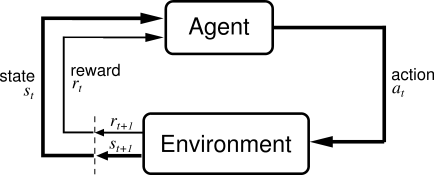
\includegraphics[scale=0.35]{figures/agent_environment_interface.png}
    \caption{Agent/Environment Interface}
    \label{fig:agent_enviroment_interface}
\end{figure}

The concept can be phrased the following way: An agent will over a series of discreet time steps $(t=1, 2, \cdots, T)$ take an action which will lead to some sort of reward (or in economic terms utility). For each time step the agent receives information about the state $S_t$ of the environment $\mathcal{E}$. The agent then takes an action $A_t$, which prompts the environment $\mathcal{E}$  to return a reward $R_{t+1}$, and a new state $S_{t+1}$. This process continues until the game terminates. The agent's sole purpose is to maximize the cumulative rewards throughout the game. It should be noted here that $R_t \in \R$ such that the agent is optimizing over a sum of scalars. The game will lead to a trajectory of states, actions and rewards that look like:

\begin{equation}
    S_0, A_0, R_1, S_1, A_1, R_2, S_2, A_2, \cdots ,R_{T-1}, S_{T-1}, A_{T-1}, R_{T}
\end{equation}

Certain assumptions is necessary to perform any sort of modelling. The most fundamental assumption reinforcement learning relies on is that of the Markov decision process: A Markov decision process (MDP) abides to:

\begin{equation}\label{eq:mdp1}
    p(s_t, r_t \mid s_{t-1},  a_{t-1}) = p(s_t, r_t \mid s_{t-1},\cdots, s_{0}, a_{t-1}, \cdots, a_{0}) = P(S_t = s_t, R_t = r_t \mid S_{t-1} = s_t, A_{t-1} = a_t)
\end{equation}

Breaking equation \eqref{eq:mdp1} down reveals that the MDP follows a true probability distribution. That is, a joint probability distribution describes $R_t$ and $S_t$. Another important feature is that the probability distribution of $S_t$ and $R_t$ only depends on the last state and action. This turns out to be an instrumental assumption for doing any sort modelling, the implication being that the state $s_t$ contains all relevant information about the past, hence the name, \textit{Markov} Decision Process. This condition/assumption yields certain important features. First, it implies that size of the probability distribution would not grow linearly as more and more states and actions was represented for the agent, yielding the computations more and more expensive. Second, it allows for backward induction and dynamic programming (a topic which will be discussed later).  Lastly one must ensure that when a system is modelled, the state represents all relevant information about the past. Multiple statements can be derived from \eqref{eq:mdp1}, but most importantly one can derive the expected reward:

\begin{equation}
    \E[R_t \mid A_{t-1} = a_{t-1}, S_{t-1} = {s_{t-1}}] = \int_{r_t} r_t \int_{s_t} p(r_t, s_t \mid a_{t-1} s_{t-1}) d s_t d r_t 
\end{equation}

The agent's goal is to maximize the cumulative rewards. This can be formulated as:

\begin{equation}\label{eq:cum_rewards}
   G_t = R_{t+1}, R_{t+2}, R_{t+3}, \cdots R_{T}
\end{equation}

The formulation in \eqref{eq:cum_rewards} can be problematic with continuing tasks. That is if $T \rightarrow \infty$. Therefore discounting of rewards is usually implemented, which have the nice economic implications, that agents in the real world tend to be impatient, and therefore more realistically model real human agents:

\begin{equation}
    G_t = R_{t+1} + \gamma R_{t+2} + \gamma^2 R_{t+3} + \cdots = \sum_{k=0}^{T - t} \gamma^k R_{t+k+1}
\end{equation}

With $\gamma$ being the discount rate, yielding a geometric series, that is known to converge, if $R_k$ is bounded.

\subsection{Value Function, Q-Function, Policy Function and the Bellman Equation}

The value function represents the expected discounted cumulative returns from following a policy, $\pi$. The value function can be said to approximate the value of a strategy:

\begin{equation}\label{eq:value_function1}
    v_{t}^{\pi}(s_t) = \E_t [G_t \mid S_t = s_t] = \E_t \lsp \sum_{k=0}^{T - t} \gamma^k R_{t+k+1} \bigg\vert S_t = s_t \rsp 
\end{equation}


A couple of things to note about \eqref{eq:value_function1}: Since the expectation is taken over a sum, one can instead take the sum over the expectations, yielding it possible to calculate the individual expected returns from following a policy, and using those to calculate the value function. Another concept that closely resembles the value-function is the Q-function:

\begin{equation}
    q_t^{\pi} (s_t, a_t) = \E_t [G_t \mid S_t = s_t, A_t = a_t ] = \E_t \lsp \sum_{k=0}^{T - t} \gamma^k R_{t+k+1} \bigg\vert S_t = s_t, A_t = a_t\rsp 
\end{equation}

The Q-function only differs from the value function by also conditioning on the action, and not only the state. The value function and the Q-function shares the property that it maps the expected value of a state (or state action pair) to a scalar value, where this value represents the cumulative, discounted rewards of following a certain policy. This has the nice property of allowing the agent to choose an action which maps to the highest expected value, $G_t$.

The Bellman equation can be expressed, using the expression for the value function:

\begin{equation}
    v^{\pi}_{t} (s_t) = \E_t [G_t \mid S_t] = \E_t  \lsp R_{t+1} + \gamma G_{t+1} \mid S_t \rsp = \E_t \lsp R_{t+1} + \gamma v_{t+1}^{\pi}(S_{t+1}) \rsp
\end{equation}

One should consider that $\E [v_{t+1}^\pi(s_{t+1})]$ does not imply $v_{t+1}^{\pi}(\E[s_{t+1}])$, which has the consequence of considerable computational markup when solving a model using the Bellman Equation as an update rule.

Lastly some information about the policy function.  A policy function defines how the agent chooses an action:

\begin{equation}
    \pi_t : \statespace \mapsto \actionspace 
\end{equation}

In general reinforcement learning algorithms falls in two distinct categories: Algorithms that directly estimate the policy function or algorithms that work by estimating the value function or Q-function, and using these to find the optimal policy. In this paper the primary focus will be on the latter category of algorithms.

\subsection{Relationship to Dynamic Programming}\label{sec:dynamic_programming}

Dynamic programming, invented by Richard Bellman, allows for a way to find the optimal policy, $\pi^{*}$, and the associated value function, $v^{\pi^{*}}$. Dynamic programming has a set of practical and formal requirements. First, the size of the state space should be limited. This is due to the fact, that number of computations will increase exponentially with the number of states, what Richard Bellman described as ``The Curse of Dimensionality''. Secondly it requires that the entire MDP is known. Here one should distinguish between an environment and a model of an environment. In this paper the model and the environment coincide, but this is not always the case. An example could be a self driving car. Because the self driving car does not have a perfect model of the environment, dynamic programming cannot be used as an algorithm for navigating the environment. In other words, unless the joint probability distribution of states and actions can be formulated explicitly, dynamic programming is not feasible. In general, it can be said that dynamic programming (and also reinforcement learning) is to use the value function to structure the search for good policies  \parencite{sutton_reinforcement_2018}.  The optimal value function  implies that one knows the optimal policy:

\begin{equation}
    v_t^{*}(s_t) = \underset{a}{\max}  \E \lsp R_{t+1} + \gamma v^{*}_{t+1}(S_{t+1}) \mid S_t = s_t, A_t = a\rsp 
\end{equation}

Dynamic programming problems can be solved by two different approaches: \textit{value function iteration} and \textit{policy function iteration}.

\textit{Policy function iteration} consists of two steps: 1) an evaluation step. Which calculates the value of a policy, and 2) a policy improvement step.
The first step can be considered a prediction step. By following a given policy the associated value function can be calculated. This is done by sweeping through the state space calculating the expected value of the state following the policy. This process continues until the algorithm has converged. In this context convergence implies the difference between the previous estimation of the value function and the current estimation of the value function, only differs below some threshold. The second step, policy improvement, works by searching through the state space, seeing if diverging from the current policy yields higher expected cumulative returns. An alternative phrasing is: Assume that the policy used for the evaluation step is optimal. Then there should be no other strategy that would yield a higher value-function for all possible states. This can be expressed more formally as:

\begin{equation}
     \E \lsp R_{t+1} + \gamma v^{*}_{t+1}(S_{t+1}) \mid S_t = s_t, A_t = \pi_t^*(s_t) \rsp \geq \E \lsp R_{t+1} + \gamma \tilde{v}_{t+1}(S_{t+1}) \mid S_t = s_t, A_t =\tilde{\pi}_t(s_t) \rsp \qquad \forall s_t \in \statespace
\end{equation}

Where $\tilde{\pi}$ is any arbitrary policy. If at any point in the state space one can find a policy that yields a higher value function than the current, then one should switch policy, which yields an updated, superior policy! The process alternates between policy evaluation and policy improvement, until no better policy can be found. A graphical representation of the process can be considered as shown in equation \eqref{eq:policyevaluation} where $\overset{\textbf{E}}{\longrightarrow}$ denotes a policy evaluation and $\overset{\textbf{I}}{\longrightarrow}$ denotes policy improvement:

\begin{equation}
    \label{eq:policyevaluation}
    \pi^0 \overset{\textbf{E}}{\longrightarrow}
    v^{\pi^0} \overset{\textbf{I}}{\longrightarrow} \pi^1 \overset{\textbf{E}}{\longrightarrow} v^{\pi^1} \overset{\textbf{I}}{\longrightarrow} \cdots \overset{\textbf{I}}{\longrightarrow} \pi^* \overset{\textbf{E}}{\longrightarrow} v^{\pi^*}
\end{equation}

The second approach \textit{value function iteration} computes a max over the value function implying only a single sweep through the state space in each iteration of the loop. The max operation yields value function iteration a considerably faster solution method. Value function iteration can be considered using the Bellman equation as an update rule \parencite{sutton_reinforcement_2018}. The algorithm for value function iteration is described below:

\begin{algorithm}[H]
\SetAlgoLined
\KwResult{Yielding $\pi^*, v^*$}
 Algorithm parameter $\theta > 0$ determining accuracy of estimation\;
 Initialize $V(s)\quad \forall s \in \statespace$ except $V(terminal) = 0$\;
 \While{$\Delta > \theta$}{
    $\Delta \la 0$ \; 
    \ForEach{$s \in \statespace$}{
        $v \la V(s)$ \;
        $V(s) \la \underset{a}{\max} \E [R_{t+1}  + \gamma V(S_{t+1}) \mid A_t = a, S_t = s] $ \;
        $\Delta \la \max (\Delta, \mid  v - V(s) \mid )$
    }
 }
 \caption{Value Function Iteration}
\end{algorithm}

 So for each sweep through the state space a single sweep of policy evaluation and a single sweep of policy improvement is performed. Again this algorithm terminates when the difference between the value function of the last sweep and the current value function is below some threshold.
 
 In economics a dynamic programming solution will usually have the addition of using backwards induction. This is due to the fact the age will evolve deterministically. The model assumes an agent acting over $T$ time steps, terminating when the agent reaches a certain age. So in a sense the agent moves in a deterministic fashion towards the termination of the environment. This implies that one can solve such a model by only doing a single sweep through the state space! The agent will maximize its value function in the terminating period. Now using this value associated with the terminating period, the agent can consider his actions in $T-1$, remembering the Bellman equation can be used as an update rule:
 
 \begin{equation}
     V_{T-1}(s_{t-1}) = \underset{a}{\max}\E [R_T + \gamma V_T (S_T) \mid S_{T-1} = s_{T-1}, A_{T-1} = a]
 \end{equation}
 
 In other words, one can model all possible states that the agent can encounter in each time step of the model, making it possible to find the optimal value function $v^{\pi^*}$ and policy function $\pi^{*}$ by a single sweep through the state space using a combination of dynamic programming and backwards induction. The implementation of value function iteration in this paper will be explored in section \ref{sec:solution_methods}. In the reinforcement learning literature, this concept of updating estimates of values of states based on value estimates of other states, is called bootstrapping\footnote{In economics bootstrapping will usually refer to a non-parametric, sample based approach for doing inference of a parameter estimate. These things are unrelated.}. 

 Before moving on to other reinforcement learning techniques, the concept of \textit{Generalized Policy Iteration} (GPI) is introduced. GPI is the concept of letting policy iteration and policy improvement interact with the intention of having the policy converge to the optimal policy. In practice the policy evaluation will be done with respect to the current policy. Policy improvement will be greedy with respect to the current value function. As described by \textcite{sutton_reinforcement_2018}: The value function stabilizes only when it is consistent with the current policy, and the policy stabilizes
only when it is greedy with respect to the current value function.
Thus, both processes stabilize only when a policy has been found that is greedy with respect to its own evaluation function. This implies that the Bellman optimality equation holds, and thus that the policy and the value function are optimal.
 
 \subsection{Overview of Reinforcement Learning Techniques}
 
Two different reinforcement learning methods will be presented in section \ref{sec:solution_methods}. Here I present some basic information that makes the reader able to digest the material presented. First it is important to address why not only use dynamic programming. Dynamic programming requires that a perfect model of the environment is accessible. This is due to the fact, that when calculating the expected value function for each action, the probability distribution of the reward and the next state, needs to formulated in an explicit form. The other techniques presented here does not have the same requirement. Secondly DP methods require that the size of the state space must be limited. The implementations presented later does not have the same requirements, allowing for approximating the value function and/or the policy function. Below I explain two different methods of learning \textit{Monte Carlo Methods} and \textit{Temporal Difference Learning} these being the two foundations of the reinforcement learning methods presented later. It is useful to distinguish between \textit{control} and \textit{prediction}. Prediction can be considered the step of estimating the value function, whereas control relates to how to approximate the optimal policies. Finally, one should make a distinction between \textit{off-policy} and \textit{on-policy} methods. \textcite{sutton_reinforcement_2018} describes the difference as: On-policy methods attempt to evaluate or improve the policy that is used to make decisions, whereas off-policy methods evaluate or improve a policy different from that used to generate the data.

\subsubsection{Monte Carlo Methods}

Before delving into MC-methods it is appropriate to introduce some more terminology: When talking about an \textit{episode} it should be understood as an agent moving through the environment from start to termination. When talking about a \textit{step} it should be understood as going from one state to the next in the environment. 

First consider the problem of Monte Carlo prediction. The best way to get a sense of prediction with Monte Carlo methods is to present an algorithm:

\begin{algorithm}[H]
\SetAlgoLined
\KwResult{Yielding $v^{\pi}$}
 Input: policy $\pi$ to be evaluated\;
 $Returns(s) \la$ an empty list $s \in \statespace$\; 
 \While{Forever}{
    Generate an episode: $S_0, A_0, R_1, S_1, A_1, \cdots S_{T-1}, A_{t-1}, R_T$\; 
    $G \la 0$ \;
    \ForEach{step in episode, $t = \{T -1 , T-2 , \cdots, 0\}$}{
        $G \la \gamma G + R_{t+1}$\;
        \If{$S_t \notin \{S_{t-1}, S_{t-2}, \cdots S_0 \}$}{
            Append $G$ to $Returns(S_t)$ \;
            $V(S_t) \la average(Returns(S_t))$ \;
        }
    }
 }
 \caption{First-Visit MC prediction, for estimating $v^{\pi}$}
 \label{alg:mcfirstvisit}
\end{algorithm}

Algorithm \ref{alg:mcfirstvisit} shows how the general concept of estimating the value function for given policy. The agent follows the policy until the game terminates. Starting from the terminating state, a reversed experience replay is performed using the discounted rewards to approximate the value function for each state the agent visited. However, the algorithm above relies on a model of the environment. If not such a model is present, one will need to estimate the value of each action. Instead of considering the value function, the Q-function (state-action pair) is used for Monte Carlo estimation. It is assumed that the policy stays constant. That is, the policy does not update as more and more episodes are experienced, which defeats the purpose of learning how to interact with the environment. This can be addressed by updating the policy, and then discard old experience. Another possibility is to accept the non-stationarity of the data collected, and update the policy using the data from a previous policy, hoping that with time the algorithm will converge. This is in fact generalized policy iteration.

Consider now how to do Monte Carlo Control, i.e., approximating the optimal policy. Just as with policy iteration the pattern followed is:

\begin{equation}
    \label{eq:montecarlocontrol}
    \pi^0 \overset{\textbf{E}}{\longrightarrow}
    q^{\pi^0} \overset{\textbf{I}}{\longrightarrow} \pi^1 \overset{\textbf{E}}{\longrightarrow} q^{\pi^1} \overset{\textbf{I}}{\longrightarrow} \cdots \overset{\textbf{I}}{\longrightarrow} \pi^* \overset{\textbf{E}}{\longrightarrow} q^{\pi^*}
\end{equation}
Policy evaluation is done as described above. Policy improvement is done by making the policy greedy with respect to the current estimated Q-function \parencite{sutton_reinforcement_2018}. Since the Q-function instead of the value function is used, no model is needed to construct a greedy policy \parencite{sutton_reinforcement_2018}. The greedy policy is the one that for each $s \in \statespace$ deterministically chooses an action with maximal action-value:

\begin{equation}
    \pi(S_t) = \underset{a}{\argmax}  Q( S_t, a )
\end{equation}

Now this algorithm rests on the assumption of \textit{exploring starts} and on the assumption of \textit{infinite episodes}. The assumption of infinite episodes is to ensure convergence, and in practice the algorithm is usually run until the algorithm has converged by some high number of episodes. The more problematic assumption is that of exploring starts. This is due to the fact, that in reality one cannot assume that there is a non-zero probability of starting in all states $s \in \statespace$, and proceed the episode from that starting point. This is an essential assumption, because otherwise, one could not know the value function of unexplored states without visiting them. 

The problem of not visiting every state is closely related to the exploration vs. exploitation trade-off. If an algorithm acts greedy (only exploits) new and better policies will never be discovered. The exploration of the state space can be done by either on-policy control or off-policy control. The exploration will in this paper be done by $\epsilon$-greedy algorithms. $\epsilon$-greedy algorithms chooses with probability $1 - \epsilon$ a (uniformly) random action each step, else it greedily chooses the action that corresponds to the highest Q-value. The next section will give an example of both on-policy and off-policy methods. 

\subsubsection{Temporal Difference Learning}

Temporal Difference (TD) learning combines ideas taken from Dynamic Programming and Monte Carlo Methods. It takes from Monte Carlo methods, that you do not need a perfect model of the environment. It takes from Dynamic Programming the bootstrapping, i.e., it uses learned estimates to update, without needing the final outcome. Just as Monte Carlo methods, Temporal difference methods has a prediction and control element.

TD prediction can be summarized in the equation:

\begin{equation}
    V(S_t) \leftarrow V(S_t) + \alpha \lsp R_{t+1} + \gamma V(S_{t+1}) - V(S_t) \rsp
\end{equation}

The equation states that $V(S_t)$ should be updated according to the return in a given period + the value function of the next period $V(S_{t+1})$. This method is called TD(0), since it only uses 1 step to update the value function. In essence TD methods learn a guess from a guess. This allows for not having a complete model of the environment (of rewards and next-state probability distributions). Compared to MC methods the TD methods can learn at each step; update its estimate at each point in time. It is also proven, that for any policy $\pi$ kept fixed, then a TD(0) algorithm will converge to $v^{\pi}$ \parencite{sutton_reinforcement_2018}. Even though, an open mathematical question, in practice it is found that TD methods converge faster than MC methods \parencite{sutton_reinforcement_2018}.

Control with temporal difference learning, can also be separated into on-policy control and off-policy control. The most used on-policy control for TD methods is called SARSA (state, action, reward, state, action). Just as with MC methods a need to trade off exploitation and exploration is present. The agent want to see new parts of the state space (exploration), but should also use (exploit) what is assumed to be the optimal choice given the value function associated with the current value function. Consider the policy generating the data being an $\epsilon$-greedy algorithm. In this case, instead of using the value function, consider the case of using the state-action pair function $Q(S_t, A_t)$, yielding the update rule:

\begin{equation}
    Q(S_t, A_t) \leftarrow Q(S_t, A_t) + \alpha \lsp R_{t+1} + \gamma Q(S_{t+1}, A_{t+1}) - Q(S_t, A_t) \rsp
\end{equation}

This update is made after each step in a non-terminal state of the environment. 
Now notice here that the update rule uses the realized state $S_{t+1}$ and $A_{t+1}$. In other words the data that is used to update the estimate is the data generated from following the epsilon greedy policy! 

Off-policy control can be done by using Q-learning. Q-learning has the slight twist on update the rule for SARSA that:

\begin{equation}
    Q(S_t, A_t) \leftarrow Q(S_t, A_t) + \alpha \lsp R_{t+1} + \gamma \underset{a}{\max} Q(S_{t + 1}, a) - Q(S_t, A_t) \rsp 
\end{equation}
Actions is still chosen by an $\epsilon$-greedy policy, the difference here being the updating rule presenting a different policy than the actual policy followed. This is due to the fact that the Q-function is updated under the assumption of greedily choosing an action in time $t+1$ conditional on the state. Q-learning and double Q-learning will be explored in depth later when describing the algorithms used in this paper.

\subsection{Landmarks}

Finally, a brief overview of environments/games where reinforcement learning have been instrumental to the current hype of reinforcement learning. The first big success of reinforcement learning was made by Tesauro in 1992 creating an agent capable of learning to play backgammon trough self play \parencite{sutton_reinforcement_2018}. Using an artificial neural network to approximate the value function, and using a temporal difference algorithm, the algorithm was capable of playing expert level backgammon. In 2011 the IBM Watson algorithm won in jeopardy using the same methods as Tesauro did for his backgammon agent \parencite{sutton_reinforcement_2018}. In 2013 the company DeepMind (now acquired by google), showed that it was possible for a reinforcement learning algorithm to learn to play video games. Here an important feat was, that it was fed the raw image input and used an artificial neural network to transform this image into a representation of the state space allowing for navigating in the environment \parencite{mnih_playing_2013}. In 2016 DeepMind created AlphaGo and a year later AlphaGo Zero, which learned to master the game of Go. This was assumed in a long time to be a hard problem for learning algorithms due to its very large state and action space \parencite{silver_general_2018}. The first iteration used expert players to learn the game, while the AlphaGo zero used only selfplay. These examples show that the capabilities of these algorithms to learn to navigate in complicated environments, might leave a way for high dimensional dynamic economic models to be solved using reinforcement learning methods.